%!TEX root = ../vernier.tex
\section{Highlighting Change} \label{sec:highlighting}
As previously mentioned, one of the reasons one might use visualization is to discover the unknown. One place that we might find interesting patterns without initially knowing what we are looking for is where most change takes place from one revision to the next. That's the reason we decided to add the option of highlighting the entities that moved the most in $\mathbb{R}^{n}$ from revision $t_{i}$ to $t_{i+1}$.

The highlight consists of a temporary aura that surrounds points in the projection and partially covers entities on the Treemap during the change of revision animation. This allows us to see where hierarchically in the project as well as in which groups in the projection coding effort has been put.

Figures \ref{fig:high_rev_22} and \ref{fig:high_rev_44} highlight the entities where most change happened in revision 22 and 44 respectively. We can see that in one a lot of change happened in small classes of one particular package (hierarchical neighbors), while in the other a lot of change took place is large classes (projection neighbors). This kind insight might be extremely valuable when trying to find the origin of a bug, for example.

\begin{figure}[H]
	\centering
	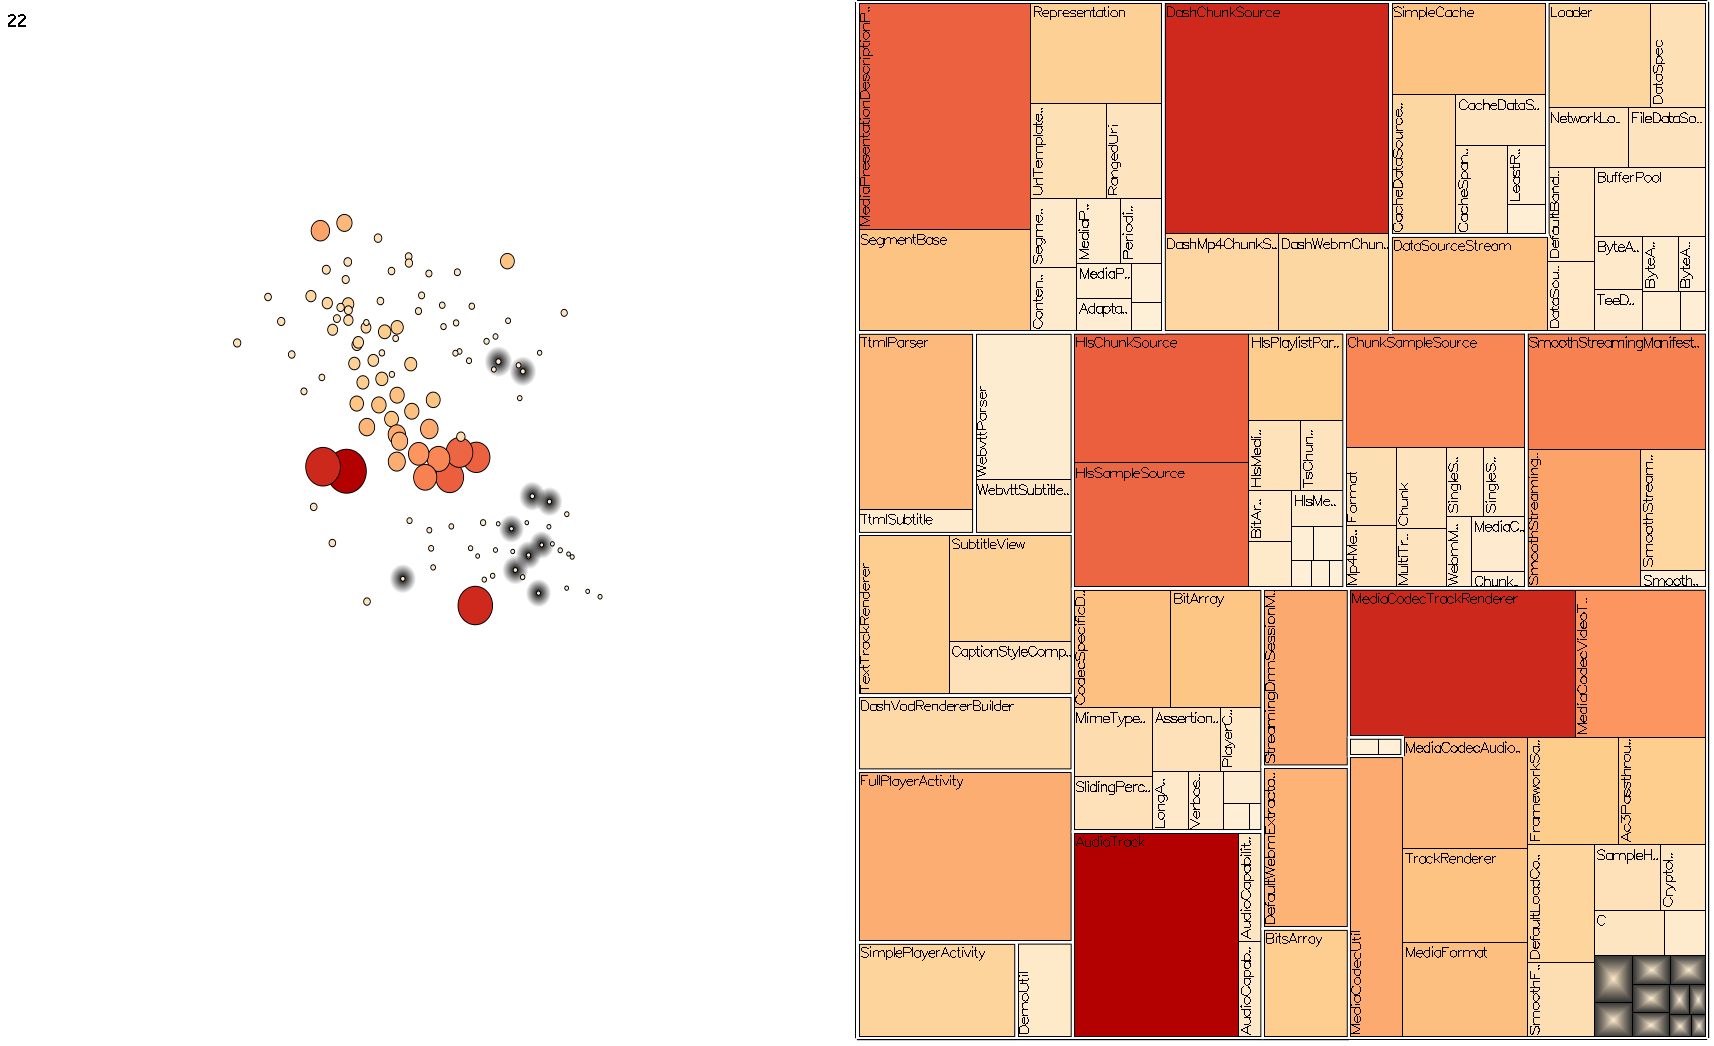
\includegraphics[width=1.0\textwidth]{figures/high_rev_22.png}
	\caption{Highlight of change in Revision 22}
	\label{fig:high_rev_22}
\end{figure}

\begin{figure}[H]
	\centering
	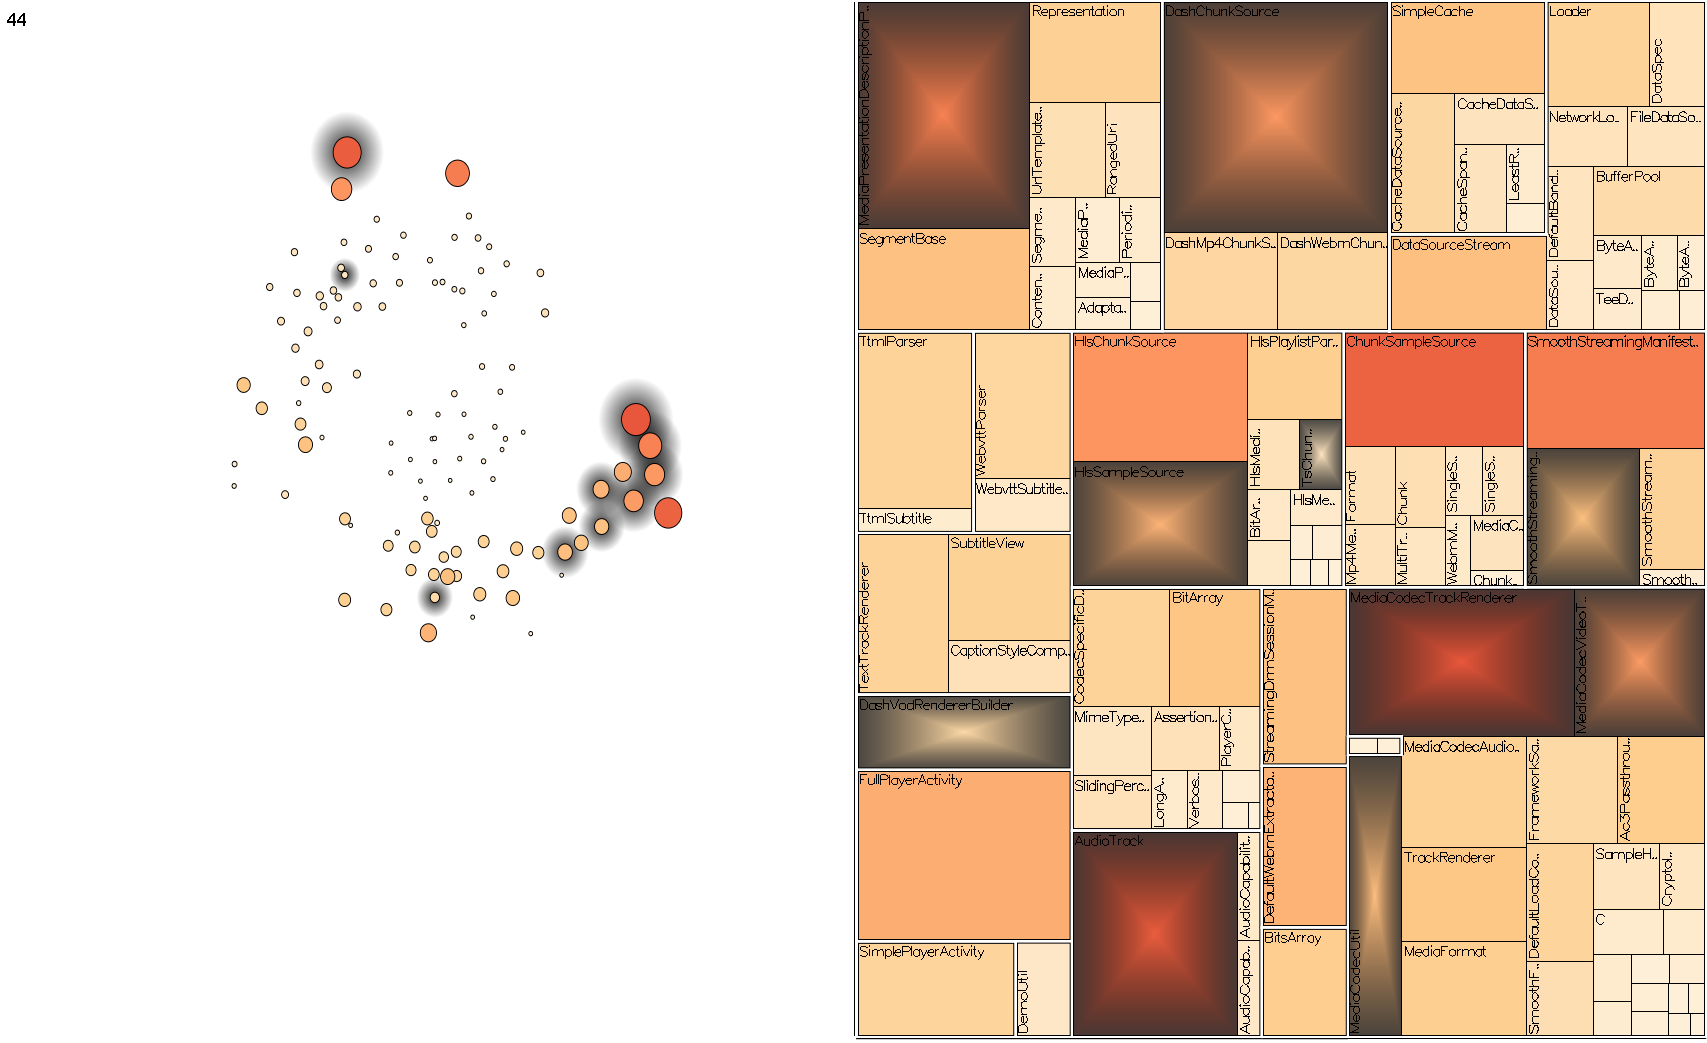
\includegraphics[width=1.0\textwidth]{figures/high_rev_44.png}
	\caption{Highlight of change in Revision 44}
	\label{fig:high_rev_44}
\end{figure}

Additionally to project information, this data could be used to "debug" the projection technique, identifying false positive (i.e. points that moved a lot in $\mathbb{R}^{2}$ but not in $\mathbb{R}^{n}$) and false negative (i.e. points that barely moved in $\mathbb{R}^{2}$ but traveled significantly in $\mathbb{R}^{n}$) errors in change.
